\documentclass[a4paper]{article}
\usepackage[14pt]{extsizes}
\usepackage{setspace,amsmath}
\usepackage{savesym}
\savesymbol{iint}
\usepackage{txfonts}
\restoresymbol{TXF}{iint}
\usepackage[left=20mm, top=20mm, right=20mm, bottom=20mm]{geometry}
\setlength{\parindent}{12,5mm}
\linespread{1.15}
\usepackage[russian]{babel}
\usepackage[T2A]{fontenc} % кодировка
\usepackage{fontspec} 
\defaultfontfeatures{Ligatures={TeX}, Renderer=Basic} 
\setmainfont[Ligatures={TeX,Historic}]{Times New Roman}
\usepackage{graphicx}
\usepackage{lscape}
\usepackage{hyperref}
\usepackage[paper=portrait,pagesize]{typearea}
\hypersetup{
    colorlinks=true,
    linkcolor=blue,
    filecolor=magenta,      
    urlcolor=cyan,
}
\graphicspath{{pictures}}
\DeclareGraphicsExtensions{.pdf,.png,.jpg}
\begin{document}
\begin{titlepage}
\begin{center}
        \large{МИНИСТЕРСТВО ОБРАЗОВАНИЯ РЕСПУБЛИКИ БЕЛАРУСЬ\\
        Белорусский Национальный Технический Университет\\
        Факультет транспортных коммуникаций\\
        Кафедра "Геодезия и аэрокосмические геотехнологии"}
    \end{center}
    \begin{center}
        \vspace{13ex}
        \large{ОТЧЁТ\\
        по лабораторной работе №3\\
        <<Уравнивание линейно-угловой сети в виде геодезического четырехугольника>>\\
        Вариант 4}
    \end{center}
    \begin{flushright}
        \vspace{13ex}
        \large{Выполнил: Вишняков М.К.,\\
        студент группы 11405118\\
        \vspace{5ex}
        Проверил: Будо А.Ю.,\\
        ст. пр. каф."ГиАКГТ"\\}
    \end{flushright}
    \begin{center}
        \vfill
        \large{Минск, 2021}
    \end{center}
\end{titlepage}
\newpage

\begin{table}[h]
    \caption{Координаты исходных пунктов}
    \centering\begin{tabular}{|p{0.17\linewidth}|p{0.17\linewidth}|p{0.17\linewidth}|}
    \hline
         $\text{Пункт}$ & $\text{N, м}$ & $\text{E, м}$\\
         \hline
         $A$ & $1088,000$ & $124,000$ \\
         \hline
         $B$ & $1614,000$ & $652,000$ \\
         \hline
    \end{tabular}
\end{table}
\begin{table}[h]
    \caption{Приближенные координаты пунктов}
    \centering\begin{tabular}{|p{0.18\linewidth}|p{0.18\linewidth}|p{0.18\linewidth}|}
    \hline
         $\text{Пункт}$ & $\text{N, м}$ & $\text{E, м}$\\
         \hline
         $C$ & $1587,000$ & $1376,000$ \\
         \hline
         $D$ & $993,000$ & $1163,000$ \\
         \hline
    \end{tabular}
\end{table}

\begin{table}[h]
    \centering
    \caption{Измеренные стороны и направления}
    \begin{tabular}{|p{3.5cm}|p{6.0cm}|}
    \hline
    \multicolumn{1}{|c|}{Элемент} & \multicolumn{1}{|c|}{Измеренные стороны, направления}\\
    \hline
    \multicolumn{2}{|c|}{Длины сторон d, м }\\
    \hline
    \multicolumn{1}{|c|}{DC} & \multicolumn{1}{c|}{810,815}\\
    \hline
    \multicolumn{2}{|c|}{Горизонтальное направление $M_i$ ,°}\\
    \hline
    \multicolumn{1}{|c|}{AB} & \multicolumn{1}{c|}{0,00000000}\\
    \hline
    \multicolumn{1}{|c|}{AC} & \multicolumn{1}{c|}{23,173277778}\\
    \hline
    \multicolumn{1}{|c|}{AD} & \multicolumn{1}{c|}{50,109166667}\\
    \hline
    \multicolumn{1}{|c|}{BC} & \multicolumn{1}{c|}{0,00000000}\\
    \hline
    \multicolumn{1}{|c|}{BD} & \multicolumn{1}{c|}{48,397638889}\\
    \hline
    \multicolumn{1}{|c|}{BA} & \multicolumn{1}{c|}{132,947888889}\\
    \hline
    \multicolumn{1}{|c|}{CD} & \multicolumn{1}{c|}{0,00000000}\\
    \hline
    \multicolumn{1}{|c|}{CA} & \multicolumn{1}{c|}{48,520166667}\\
    \hline
    \multicolumn{1}{|c|}{CB} & \multicolumn{1}{c|}{72,399861111}\\
    \hline
    \multicolumn{1}{|c|}{DA} & \multicolumn{1}{c|}{0,00000000}\\
    \hline
    \multicolumn{1}{|c|}{DB} & \multicolumn{1}{c|}{45,340000000}\\
    \hline
    \multicolumn{1}{|c|}{DC} & \multicolumn{1}{c|}{104,5421666673}\\
    \hline
\end{tabular}
\end{table}
\newpage
\par
\large{
СКП измеренных расстояний вычисляют по формуле:

\begin{equation}
    m = a + b \cdot D
\end{equation}

где $a$ = 3 мм , $b$ = 0,000005 мм
\par
Выполнив расчет, получили, что СКП измеренных расстояний равно: $m$ = 0,070541 дм.
\par
СКП угла тахеометра: $m_\beta = 2"$. СКО горизонтальных направлений:

\begin{equation}
    m_M = \frac{m_\beta}{\sqrt{2}}
\end{equation}

\begin{table}[h]
    \centering
    \caption{СКО горизонтальных направлений}
    \begin{tabular}{|p{3.5cm}|p{6.0cm}|}
        \hline
         $\text{Направления}$ & $\text{СКО направления}, "$\\
         \hline
         AB & 1,4142 \\
         \hline
         AC & 1,4142 \\ 
         \hline
         AD & 1,4142 \\ 
         \hline
         BC & 1,4142 \\ 
         \hline
         BD & 1,4142 \\ 
         \hline
         BA & 1,4142 \\ 
         \hline
         CD & 1,4142 \\ 
         \hline
         CA & 1,4142 \\ 
         \hline
         CB & 1,4142 \\ 
         \hline
         DA & 1,4142 \\ 
         \hline
         DB & 1,4142 \\ 
         \hline
         DC & 1,4142 \\ 
         \hline
    \end{tabular}
    
\end{table}
}
\par
\large{Далее составляется матрица \textit{P}, т.е. матрицы весов измерений размерности $N\times N$
\begin{equation}
    P_i=\frac{1}{m_i^2}
\end{equation}
где $P_i$ $-$ вес $\textit{i}$-го расстояния или горизонтального направления.\\
$m_i -$ СКО измеренных расстояний или горизонтальных направлений.
\par Сама матрица имеет следующий вид, представленный в \hyperlink{add_1}{Приложении 1}
\par Затем составляют матрицу коэффициентов параметрических уравнений
поправок. Для этого заполняют матрицу частными производными по всем измерениям, по следующим формулам:
\begin{equation}
    a_{ik} = -\rho\cdot\frac{E_k-E_i}{S^2}
\end{equation}
\begin{equation}
    b_{ik} = \rho\cdot\frac{N_k-N_i}{S^2}
\end{equation}
\begin{equation}
   S^2 = (N_k-N_i)^2+(E_k-E_i)^2
\end{equation}
\par По вышеприведенным формулам находят поправки для измеренных направлений.
\par Поправки для измеренных расстояний находятся по следующим формулам:
\begin{equation}
    c_{ik} = \frac{E_k-E_i}{S}
\end{equation}
\begin{equation}
    d_{ik} = \frac{N_k-N_i}{S}
\end{equation}
\begin{equation}
   S = \sqrt{(N_k-N_i)^2+(E_k-E_i)^2}
\end{equation}}
\small{
\begin{center}
    $A =
    \begin{bmatrix}
        0 & 0 & 0 & 0 & -1 & 0 & 0 & 0 \\
        -14,216505731 & 5,666163226 & 0 & 0 & -1 & 0 & 0 & 0 \\
        0 & 0 & -19,687650654 & -1,800122052 & -1 & 0 & 0 & 0 \\
        -28,450047099 & -1,060982419 & 0 & 0 & 0 & -1 & 0 & 0 \\
        0 & 0 & -16,296770063 & -19,804881035 & 0 & -1 & 0 & 0 \\
        0 & 0 & 0 & 0 & 0 & -1 & 0 & 0 \\
        -11,033112023 & 30,768396909 & 11,033112023 & -30,768396909 & 0 & 0 & -1 & 0 \\
        -14,216505731 & 5,666163226 & 0 & 0 & 0 & 0 & -1 & 0 \\
        -28,450047099 & -1,060982419 & 0 & 0 & 0 & 0 & -1 & 0 \\
        0 & 0 & -19,687650654 & -1,800122052 & 0 & 0 & 0 & -1 \\
        0 & 0 & -16,296770063 & -19,804881035 & 0 & 0 & 0 & -1 \\
        -11,033112023 & 30,768396909 & 11,033112023 & -30,768396909 & 0 & 0 & 0 & -1 \\
        0,941310906 & 0,337540780 & -0,941310906 & -0,338 & 0 & 0 & 0 & 0 \\
    \end{bmatrix}$
\end{center}
}
\large{
\par Далее необходимо составить вектор свободных членов для измеренных расстояний и направлений. 
\par Для расстояний:
\begin{equation}
    l = d_{0} - d
\end{equation}
$d_0$ $-$ вычисленное расстояние между пунктами с помощью с помощью обратной геодезической задачи.\\
$d$ $-$ измеренное расстояние между пунктами.\par
Для вычисления вектора свободных членов для измеренных направлений необходимо рассчитать на каждой станции ориентирующий угол нулевого направления.\par 
Для вычисления ориентирующего угла ($\alpha_{ik}$) нужно предварительно рассчитать значения румба (\textit{r}) 
\begin{equation}
r_{ik} = \arctan\bigg{(}\frac{E_k-E_i}{N_k-N_i}\bigg{)}
\end{equation}
\par Далее анализируют в какой четверти лежит румб и в зависимости от четверти прибавляют константу $\Delta$.
\begin{equation}
    \alpha_{ik} = r_{ik} + \Delta
\end{equation}
$\Delta$ = 0 для I четверти;\\
$\Delta$ = 180 для II и III четверти;\\
$\Delta$ = 360 для IV четверти.
\par Теперь, рассчитав все необходимое, можно найти ориентирующий угол нулевого направления. Для этого стоит воспользоваться следующей формулой:
\begin{equation}
    Z_0=\frac{(\alpha_1-M_1) + (\alpha_2-M_2) + ... + (\alpha_i-M_i)}{N}
\end{equation}
}
\large{
где $\alpha_1$ $-$ вычисленный дирекционный угол
\par $M_1$ $-$ измеренное направление
\par Затем вычисляют значения направлений $M_0$:
\begin{equation}
\begin{matrix}
    M_{01} = \alpha_1 - Z_0 \\
    M_{02} = \alpha_2 - Z_0 \\
    ..... \\
    M_{0n} = \alpha_n - Z_0\\
\end{matrix}
\end{equation}
\par После этого вычисляют векторы свободных членов:
\begin{equation}
L=
\begin{bmatrix}
    M_{01} - M_1  \\
    M_{02} - M_2 \\
    ..... \\
    M_{0n} - M_n\\
\end{bmatrix}
\end{equation}
\hfill \break
\par По результатам всех вышеперечисленных вычислений получаем матрицу $L$ :
\begin{center}
$L$ =
    \begin{bmatrix}
        7,18499799 \\
        -37,31250101 \\
        30,12750302 \\
        -50,29859213 \\
        10,23613627 \\
        40,06245587 \\
        -37,33201519 \\
        43,14778190 \\
        -5,81576671 \\
        64,06287658 \\
        13,39405075 \\
        -77,45692733 \\
        3,54864330 \\
    \end{bmatrix}
\end{center}
}
\large{Теперь вычисляем вектор поправок в приближенные значения параметров. Для этого используем формулу:

\begin{equation}
    \delta = - (A^TPA)^{-1}A^TPL
\end{equation}

\par В результате:

\begin{center}
$\delta$ =
    \begin{bmatrix}
        -0,3181 \\
        -0,0357 \\
        0,1401 \\
        -0,2653 \\
        6,8018 \\
        40,2032 \\
        85,0953 \\
        42,7048 \\
    \end{bmatrix}
\end{center}

\par Прибавляя значения из вектора поправок к приближенным значениям соответствующих параметров, записываем уравненные координаты по результатам первой итерации (таблица 5).
\begin{table}[h]
    \centering
    \caption{Уравненные значения после I итерации}
    \begin{tabular}{|c|c|c|c|c|}
        \hline
        \multicolumn{3}{|c|}{До уравнивания} & \multicolumn{2}{|c|}{После      уравнивания}\\
        \hline
        Пункт & N, м & E, м & N, м & E, м\\
        \hline
        A & 1088,000 & 124,000 & 1088,000 & 124,000\\
        \hline
        B & 1614,000 & 652,000 & 1614,000 & 652,000\\
        \hline
        C & 1587,000 & 1376,000 & 1586,682 & 1375,964\\
        \hline
        D & 993,000 & 1163,000 & 993,140 & 1162,735\\
        \hline
    \end{tabular}
\end{table}

\par Процесс повторяется, но в качестве координат приближенных пунктов принимают координаты полученные после первой итерации.
\par Итерации повторяем до того момента, пока поправки в координаты приближенных пунктов не станут меньше 0,00000001 м. 
}
\large{ В результате, было выполнено четыре итерационных процесса. 
\par Окончательные координаты приближенных пунктов представлены в таблице 6.
\begin{table}[h]
    \centering
    \caption{Окончательные координаты пунктов}
    \begin{tabular}{|p{3.5cm}|p{3.0cm}|p{3.0cm}|}
    \hline
        Пункт & N, м & E, м\\
        \hline
        A & 1088,000000 & 124,000000\\
        \hline
        B & 1614,000000 & 652,000000\\
        \hline
        C & 1586,681870 & 1375,964085\\
        \hline
        D & 993,140079 & 1162,734744\\
        \hline
    \end{tabular}
\end{table}

\newpage

\begin{center}
    \Large{\textbf{Оценка точности}}
\end{center}

\par Вычислим СКП единицы веса по формуле:
    \begin{equation}
        \mu = \sqrt{\frac{V^TPV}{N - u}}
    \end{equation}
где $N$ $-$ число измерений;\\
$u$ $-$ число определяемых параметров.
\par Результат вычислений:

\begin{center}
    $V^{T}PV$ = 4,030934\\
    $N$ = 13\\
    $u$ = 8\\
    $\mu$ = 0,897879
\end{center}

\par Ковариационная матрица определяемых параметров:
    \begin{equation}
        Q = \left( A^TPA \right)^{-1}
    \end{equation}
\par Ковариационная матрица измерений:
\begin{equation}
  Q_y = A \cdot Q \cdot A^T  
\end{equation}
}
\par\large{Результаты вычислений представлены в \hyperlink{add_2}{Приложении 2} и в \hyperlink{add_3}{Приложении 3}.
\par Далее вычисляем СКП уравненных превышений:
\begin{equation}
    m_i = \mu \cdot \sqrt{Q_{i,i}}
\end{equation}

\begin{center}
    Таблица 7 $-$ Вычисленные значения\\
\begin{tabular}{|c|c|c|c|}
\hline
    $m(N_C)$ & $m(E_C)$ & $m(E_C)$ & $m(E_D)$ \\
    \hline
   0,00652 м  & 0,00864 м & 0,00684 м & 0,00691 м\\
   \hline
\end{tabular}
\end{center}

\par Теперь вычисляем СКП уравненных измерений:
\begin{equation}
    m_{Yi} = \mu \cdot \sqrt{Q_{Yi,i}}
\end{equation}
\par Вычисленные значения:
\begin{center}
    $
    m(M_{AB}) = 0,119805 \ " \\
    m(M_{AC}) = 0,110476 \ " \\
    m(M_{AD}) = 0,120899 \ " \\
    m(M_{BC}) = 0,141659 \ " \\
    m(M_{BD}) = 0,139486 \ " \\
    m(M_{BA}) = 0,142984 \ " \\
    m(M_{CD}) = 0,140208 \ " \\
    m(M_{CA}) = 0,111969 \ " \\
    m(M_{CB}) = 0,130195 \ " \\
    m(M_{DA}) = 0,124342 \ " \\
    m(M_{DB}) = 0,127950 \ " \\
    m(M_{DC}) = 0,143545 \ " \\
    m(S_{BD}) = 0,006693 \ $м$ $ 
\end{center}

\begin{center}
    \Large{\textbf{Расчет эллипсов ошибок }}
\end{center}
\par Для расчёта параметров эллипсов ошибок вычислим
вспомогательную величину $W$:
\begin{equation}
    W = \sqrt{\left(Q_{i,i} - Q_{i+1,i+1}\right)^2 + 4 \cdot \left(Q_i,i + 1 \right)^2 }
\end{equation}
\par Угол поворота большой полуоси эллипса относительно
направления на север:
\begin{equation}
    \phi = \frac{\pi}{2} - \frac{1}{2} \cdot \arcsin \left({\frac{2 \cdot Q_{i,i+1}}{W}} \right)
\end{equation}
\par Большая полуось эллипса ошибок:
\begin{equation}
    a = \mu \cdot \sqrt{\frac{Q_{i,i} + Q_{i+1,i+1} + W}{2}}
\end{equation}
\par Малая полуось эллипса ошибок:
\begin{equation}
    b = \mu \cdot \sqrt{\frac{Q_{i,i} + Q_{i+1,i+1} - W}{2}}
\end{equation}
\par Значение параметров ошибок:

\begin{table}[h]
    \centering
    \caption{Значение параметров ошибок}
    \begin{tabular}{|c|c|c|}
    \hline
        Параметр & C & D \\
        \hline
        W & 0,000370 & 0,000189 \\
        \hline
        $\phi$ & 112,821393 & 105,379649 \\
        \hline
        a & 0,007087 & 0,006123 \\
        \hline
        b & 0,004518 & 0,004719 \\
        \hline
    \end{tabular}
\end{table}

\begin{center}
    \Large{{\textbf{Статистический тест Хи-квадрат}}}
\end{center}
\par Для того чтобы в Excel выполнить статистический тест необходимо воспользоваться следующими командами: 
\begin{center}
    $\chi^{2}_1$ = ХИ.ОБР($\frac{q}{2};r$)\\
    $\chi^{2}_2$ = ХИ.ОБР($1-\frac{q}{2};r$)\\
    $\chi^{2}_1 = 0,831212$\\
    $\chi^{2}_2 = 12,832502$
\end{center}
\par Далее необходимо выполнить следующие вычисления:
$$\sqrt{\frac{\chi^{2}_1}{r}}\leq\mu\leq\sqrt{\frac{\chi^{2}_2}{r}}$$
\par Результаты вычислений:
$$\sqrt{\frac{\chi^{2}_1}{r}} = 0,407728$$
$$\sqrt{\frac{\chi^{2}_2}{r}} = 1,602030$$
$$0,407728\leq0,897879\leq1,602030$$
\par \textit{Вывод}: как итог мы наблюдаем, что статистический тест выполняется. 
}
\newpage

\KOMAoptions{paper=landscape,pagesize}
\recalctypearea
\begin{center}
\hypertarget{add_1}{\textbf{ПРИЛОЖЕНИЕ 1}}
\vfill
\vfill
    \makebox[\textwidth]{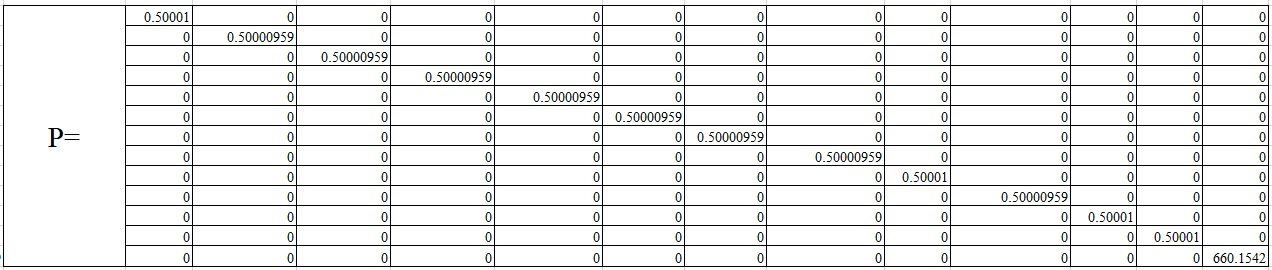
\includegraphics[width=27cm]{images/1.jpg}}
\end{center}

\newpage

\KOMAoptions{paper=landscape,pagesize}
\recalctypearea
\begin{center}
\hypertarget{add_2}{\textbf{ПРИЛОЖЕНИЕ 2}}
\vfill
\vfill
    \makebox[\textwidth]{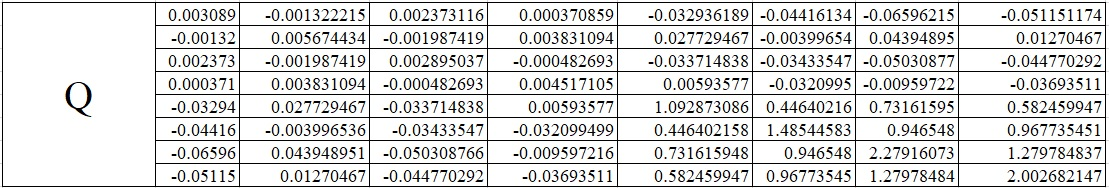
\includegraphics[width=27cm]{images/2.jpg}}
\end{center}

\newpage

\KOMAoptions{paper=landscape,pagesize}
\recalctypearea
\begin{center}
\hypertarget{add_3}{\textbf{ПРИЛОЖЕНИЕ 3}}
\vfill
\vfill
    \makebox[\textwidth]{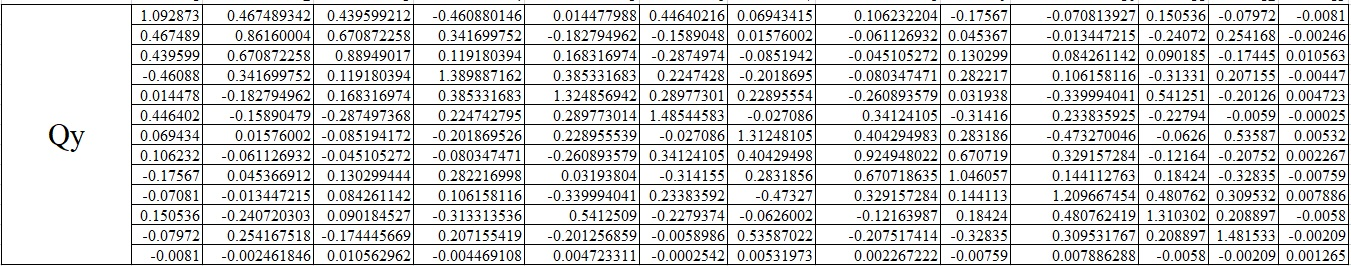
\includegraphics[width=27cm]{images/3.jpg}}
\end{center}

\end{document}